\documentclass[]{report}
\usepackage{graphicx} %buat insert gambar
\usepackage[numbered,framed]{matlab-prettifier}

\usepackage[utf8]{inputenc}
\usepackage[english]{babel}
%\usepackage[utf8]{inputenc}
\usepackage[colorlinks = true,
linkcolor = blue,
urlcolor  = blue]{hyperref}
\usepackage[a4paper,margin=1.25in]{geometry}
\usepackage{stackengine,graphicx}
\usepackage{fancyhdr}
\setlength{\headheight}{15pt}
\usepackage{microtype}
\usepackage{times}
\usepackage{booktabs}
\usepackage[numbers,sort,compress]{natbib}% numbers,sort&compress
\usepackage[section]{placeins}
\usepackage{afterpage}

% Title Page
%\title{DIGITAL SIGNAL PROCESSING}
%\author{}


\begin{document}
%\maketitle

\begin{titlepage}
	   \begin{center}
		% judul thesis harus dalam 14pt Times New Roman
		{\large\textbf{DIGITAL SIGNAL PROCESSING }} \\[1.0cm]
		\textbf{LABORATORIUM MODULES}\\
		
		\vspace*{2.0cm}
		
		\begin{figure}[h!]
			\centering 
			
\includegraphics[height=8cm,width=10cm]{logo-ub.jpg}  	
		\end{figure}
		\vspace*{4.0cm}
		
		\textbf{
			INFORMATICS STUDY PROGRAM\\
			FACULTY OF ENGINEERING AND COMPUTER SCIENCE \\
			BAKRIE UNIVERSITY\\
			JAKARTA\\
			2019\\}
	\end{center}
\end{titlepage}

\tableofcontents
\clearpage
\newpage

\chapter{Introduction to MATLAB $_{(Pt.1)}$}
\section{Objectives}
	\par After a practicum assignment, it is expected that:	
	\begin{enumerate}
		\item Recognize the environment in the MATLAB program
		\item Students can understand some of the main functions that exist in MATLAB		
	\end{enumerate}

\section{Theory}
	\par The name MATLAB stands for MATrix LABoratory. MATLAB was written originally to provide easy access to matrix software developed by the LINPACK (linear system package) and EISPACK (Eigen system package) projects. MATLAB [1] is a high-performance language for technical computing. It integrates computation, visualization, and programming environment. Furthermore, MATLAB is a modern programming language environment: it has sophisticated data structures, contains built-in editing and debugging tools, and supports object-oriented programming. These factors make MATLAB an excellent tool for teaching and research. It has powerful built-in routines that enable a very wide variety of computations. It also has easy to use graphics commands that make the visualization of results immediately available. Specific applications are collected in packages referred to as toolbox. There are toolboxes for signal processing, symbolic computation, control theory, simulation, optimization, and several other fields of applied science and engineering.

\section{Starting Matlab}
	\par When you start MATLAB, a special window called the MATLAB desktop appears. The desktop is a window that contains other windows. The major tools within or accessible from the desktop are: 
	\begin{enumerate}
		\item The Command Window 
		\item The Command History 
		\item The Workspace 
		\item The Current Directory 
		\item The Help Browser 	
	\end{enumerate}

	\begin{figure}[!t]	
		\centering
		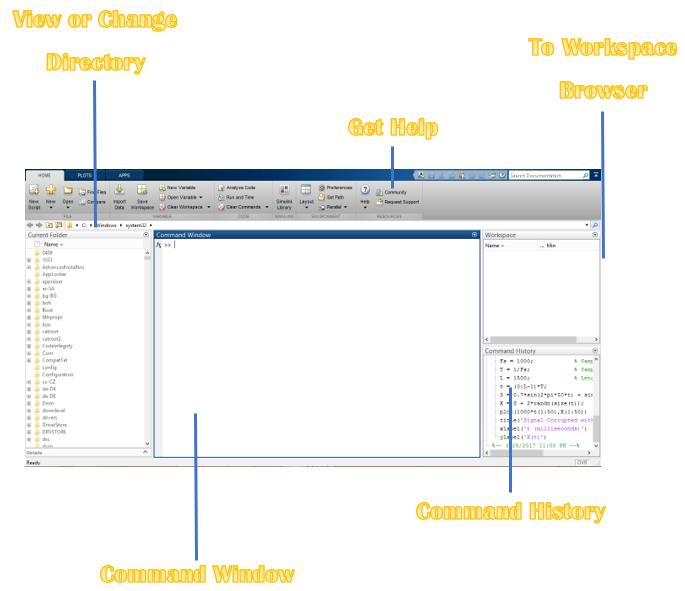
\includegraphics[height=10cm,width=13cm]{startmatlab}
		\caption{Starting Matlab}
		\label{fig:startmatlab}
	\end{figure}

\section{Creating Simple Plots $_{(Cont.)}$}
	\par 
	The basic MATLAB graphing procedure, for example in 2D, is to take a vector of x-coordinates, x = (x1, . . ., xN ), and a vector of y-coordinates, y = (y1, . . . , yN ), locate the points (xi , yi), with i = 1, 2, . . . , n and then join them by straight lines. You need to prepare x and y in an identical array form; namely, x and y are both row arrays or column arrays of the same length.
	The MATLAB command to plot a graph is plot(x,y). 
	\par The vectors x = (1, 2, 3, 4, 5, 6) and 	y = (3, $-{1}$, 2, 4, 5, 1). 
	\par The MATLAB command to plot the Vectors is;	
	\begin{lstlisting}[style=Matlab-editor]
	x = [1 2 3 4 5 6]; 
	y = [3 -1 2 4 5 1]; 
	plot (x, y) 
	\end{lstlisting}

	\par The command will show a Signal Chart like figure \ref{fig:startmatlab2}.
	\begin{figure}[!t]
		\centering
		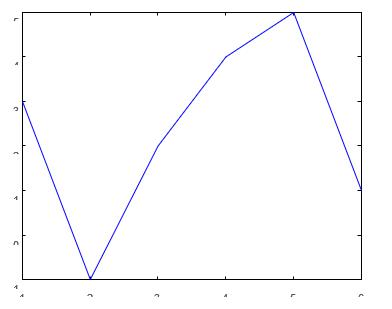
\includegraphics[height=8cm,width=10cm]{startmatlab2}
		\caption{Signal Chart}
		\label{fig:startmatlab2}
	\end{figure}
	
\section{Assignment}
	\begin{enumerate}
		\item Have you understand the basic Function of MATLAB Program(yes/no)?
		\item Make your Conclusion about MATLAB Program!	
		\item Put the picture of your first matlab code and give a brief explanation of the picture ! 
	\end{enumerate}

\section{Notes}
	\par Please write down your written task using Microsoft Word (format: DSP\_LAB1\_studentID.doc or docx) and the matlab code with the same name (format: DSP\_LAB1\_studentID.m ). The tasks must be finished at lab (no take home lab task), late submission of works will not be marked.
        

%%%%%%%%%%%%%%%%%%%%%%%%%%%%%%%%%%%%%%%%%%%%%%%%%%%%%%%%%%%%%%%%%%%%%%%%%%%%%%%%%%%%%%%%%%%%%%%%%%%%%%%%%%%%%%%%%%%%%%

\chapter{Introduction to MATLAB $_{(Pt.2)}$}
\section{Objectives}
	\par 
	After a practicum assignment, it is expected that:	
	\begin{enumerate}
		\item Students can Understand the meaning of Sine and Cosine Wave.
		\item Students can implement the Sine and Cosine formula into MATLAB Command.
		\item Students can Represent the output Signal of Sine and Cosine Wave using MATLAB Program.		
	\end{enumerate}

\section{Theory}
	\subsection{Sine Wave}
		\par 
		A sine wave or sinusoid is a mathematical curve that describes a smooth repetitive oscillation. A sine wave is a continuous wave. It is named after the function sine, of which it is the graph. It occurs often in pure and applied mathematics, as well as physics, engineering, signal processing and many other fields. Its most basic form as a function of time (t) is: \\ 
		\begin{center}
			$ y(t)=Asin(2\pi f t + \varphi ) = Asin(\omega t + \varphi) $
		\end{center}
			
		where
		\begin{itemize}
			\item A = the amplitude, the peak deviation of the function from zero.
			\item f = the ordinary frequency, the number of oscillations (cycles) that occur each second of time.
			\item $ \omega = 2 \phi f $, the angular frequency, the rate of change of the function argument in units of radians per second
			\item $\varphi$ = the phase, specifies (in radians) where in its cycle the osciWllation is at t = 0.
			\item When $\varphi$ is non-zero, the entire waveform appears to be shifted in time by the amount $\varphi/\omega$ seconds. A negative value represents a delay, and a positive value represents an advance.
		\end{itemize}

	\subsection{Cosine Wave}
		\par 
		A cosine wave is a signal waveform with a shape identical to that of a sine wave , except each point on the cosine wave occurs exactly 1/4 cycle earlier than the corresponding point on the sine wave. A cosine wave and its corresponding sine wave have the same frequency, but the cosine wave leads the sine wave by 90 degrees of phase.
		\begin{figure}[!t]
			\centering
			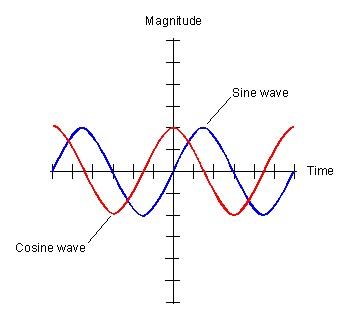
\includegraphics[height=6cm,width=6cm]{cosineWave.jpg}
			\caption{Cosine Wave}
			\label{fig:cosinewave}
		\end{figure}

\section{Sine and Cosine Wave $_{(Cont.)}$}
	\par 
	Creating a sine wave
\begin{lstlisting}[style=Matlab-editor]
x = 0:pi/100:2*pi; 
y = sin(x); 
plot (x, y) 
\end{lstlisting}
	
	\par The semicolon [:] in there means 'until'. For example, where the x stand for (0,0.1,0.2,... 5) the formula written x=0:0.1:5
	\begin{figure}
		\centering
		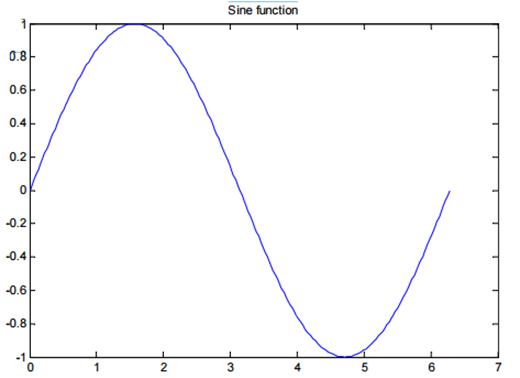
\includegraphics[height=7cm,width=8cm]{exsinwave}
		\caption{Sine Wave Example}
		\label{fig:exsinwave}
	\end{figure}

\section{Assignment}
\begin{enumerate}
	\item What is the output signal from Sine Wave below ?
	\begin{figure}
		\centering
		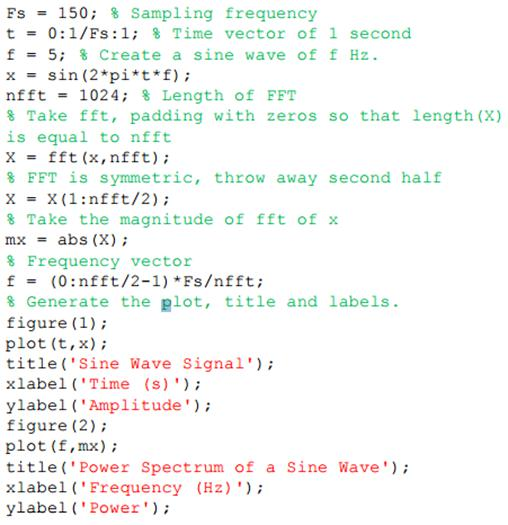
\includegraphics{lab2-code1}
		\caption{Code Assignment 1}
		\label{fig:lab2-code1}
	\end{figure}
	
	\item What is the output signal from Cosine Wave below ?	
	\begin{figure}
		\centering
		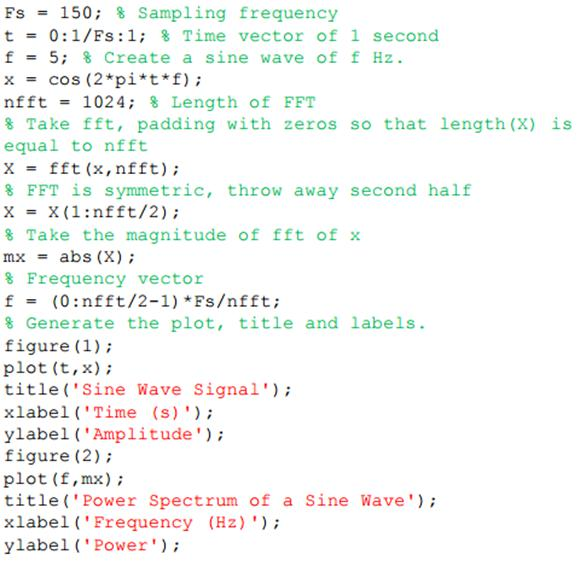
\includegraphics{lab2-code2}
		\caption{Code Assignment 2}
		\label{fig:lab2-code2}
	\end{figure}
	
	\item Make your Conclusion about Lab Practice you did today!
\end{enumerate}

\section{Notes}
	\par 
	Please write down your written task using Microsoft Word (format: DSP\_LAB2\_studentID.doc or docx) and the matlab code with the same name (format: DSP\_LAB2\_studentID.m ). The tasks must be finished at lab (no take home lab task), late submission of works will not be marked.
	     

%%%%%%%%%%%%%%%%%%%%%%%%%%%%%%%%%%%%%%%%%%%%%%%%%%%%%%%%%%%%%%%%%%%%%%%%%%%%%%%%%%%%%%%%%%%%%%%%%%%%%%%%%%%%%%%%%%%%%%

\chapter{Square Wave Signal}
\section{Objectives}
	\par After a practicum assignment, it is expected that:	
	\begin{enumerate}
		\item Students can Understand the meaning of Square Wave.
		\item Students can implement the Square Wave formula into MATLAB Command.
		\item Students can Represent the output Signal of Square Wave using MATLAB Program.
	\end{enumerate}

\section{Theory}
	\par 
	A square wave is a non-sinusoidal periodic waveform (which can be represented as an infinite summation of sinusoidal waves), in which the amplitude alternates at a steady frequency between fixed minimum and maximum values, with the same duration at minimum and maximum. The transition between minimum to maximum is instantaneous for an ideal square wave; this is not realizable in physical systems. Square waves are often encountered in electronics and signal processing. Its stochastic counterpart is a two-state trajectory. A similar but not necessarily symmetric wave, with arbitrary durations at minimum and maximum, is called a pulse wave (of which the square wave is a special case).
	
	\par 
	The square wave in mathematics has many definitions, which are equivalent except at the discontinuities:
	
	\par 
	It can be defined as simply the sign function of a periodic function, an example being a sinusoid:
	\begin{equation}
		x(t) = sgn(sin[t])\\
		v(t) = sgn(cos[t])
	\end{equation}
	which will be 1 when the sinusoid is positive, $-{1}$ when the sinusoid is negative, and 0 at the discontinuities. Any periodic function can substitute the sinusoid in this definition.


\section{Square Wave Signal $_{(Cont.)}$}
	\par To create square wave from sine wave, t must be define first.
\begin{lstlisting}[style=Matlab-editor]
t = 0:.1:.10; 
y = sin(t); 
plot (t, y) 
\end{lstlisting}

	\par The output signal is :
	\begin{figure}
		\centering
		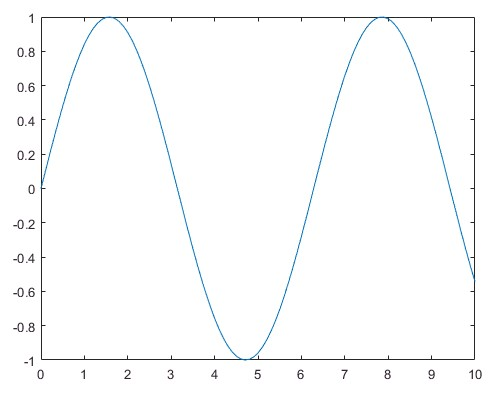
\includegraphics[height=7cm,width=8cm]{squarewave-1.jpg}
		\caption{Square Wave Signal 1}
		\label{fig:sqw1}
	\end{figure}
	\par Now, you need to translate this formula to MATLAB Command : \\ $ y= sin(t) + sin(\frac{nt}{n}) $\\If we suppose that n=3, so
\begin{lstlisting}[style=Matlab-editor]
y=sin(t) + sin(3*t)/3;
plot(t,y);
\end{lstlisting}

	\begin{figure}
		\centering
		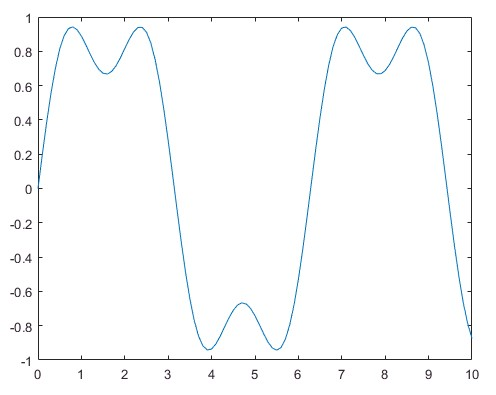
\includegraphics[height=7cm,width=8cm]{squarewave-2.jpg}
		\caption{Square Wave Signal 2}
		\label{fig:sqw2}
	\end{figure}

\section{Assignment}
	\begin{enumerate}
		\item Convert these Square Wave (from Sine Wave) Formula into MATLAB Command!
		\begin{itemize}
			\item $ y= sin(t) + sin(\frac{5t}{5}) + sin(\frac{7t}{7}) $
			\item $ y= sin(t)  + sin(\frac{3t}{3}) + sin(\frac{5t}{5}) + sin(\frac{7t}{7})  + sin(\frac{9t}{9})$
		\end{itemize}	
		
		\item What is the output signal from Cosine Wave below ?	
		\begin{itemize}
			\item See figure \ref{fig:sqwa1}
			\begin{figure}
				\centering
				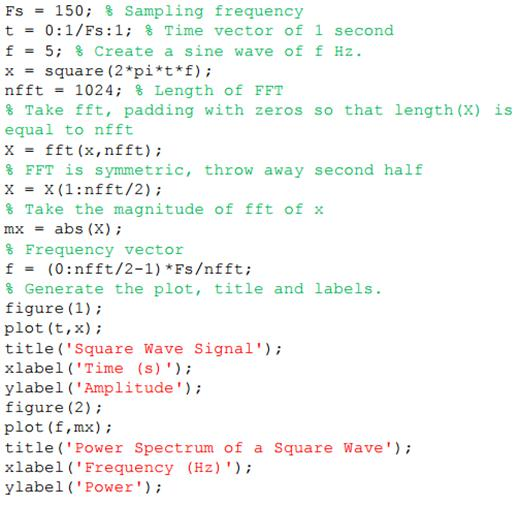
\includegraphics{sqwa1}
				\caption{Code Assignment 1}
				\label{fig:sqwa1}
			\end{figure}
			
			\item See figure \ref{fig:sqwa2}
			\begin{figure}
				\centering
				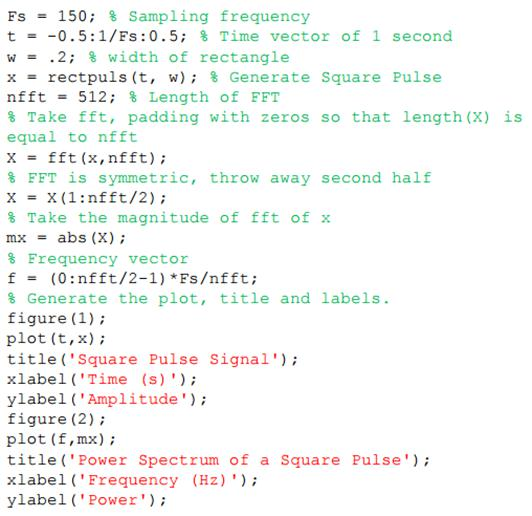
\includegraphics{sqwa2}
				\caption{Code Assignment 2}
				\label{fig:sqwa2}
			\end{figure}
		\end{itemize}	
	
		\item Make your Conclusion about Lab Practice you did today!
	\end{enumerate}

\section{Notes}
\par Please write down your written task using Microsoft Word (format: DSP\_LAB3\_studentID.doc or docx) and the matlab code with the same name (format: DSP\_LAB3\_studentID.m ). The tasks must be finished at lab (no take home lab task), late submission of works will not be marked.


%%%%%%%%%%%%%%%%%%%%%%%%%%%%%%%%%%%%%%%%%%%%%%%%%%%%%%%%%%%%%%%%%%%%%%%%%%%%%%%%%%%%%%%%%%%%%%%%%%%%%%%%%%%%%%%%%%%%%%

\chapter{Sawtooth Wave Signal}
\section{Objectives}
	\par 
	After a practicum assignment, it is expected that:	
	\begin{enumerate}
		\item Students can Understand the meaning of Sawtooth Wave.
		\item Students can implement the Sawtooth Wave formula into MATLAB Command.
		\item Students can Represent the output Signal of Sawtooth Wave using MATLAB Program.
	\end{enumerate}

\section{Theory}
	\par 
	The sawtooth wave (or saw wave) is a kind of non-sinusoidal waveform. It is so named based on its resemblance to the teeth of a plain-toothed saw with a zero rake angle.
	The convention is that a sawtooth wave ramps upward and then sharply drops. However, in a "reverse (or inverse) sawtooth wave", the wave ramps downward and then sharply rises. It can also be considered the extreme case of an asymmetric triangle wave. \\

	\par 
	The piecewise linear function
	\begin{equation}
		x(t) = t - [t] = t - floor(t)
	\end{equation}
	
	\begin{center}
		or
	\end{center}

	\begin{equation}
		x(t) = t(mod1)
	\end{equation}

	\par
	T is an example of a sawtooth wave with period 1 based on the floor function of time t. A more general form is in the range of -1 to 1 and in the period a
	\begin{equation}
		x(t) = 2 (\frac{t}{a} - [\frac{1}{2} + \frac{t}{a}]) = 2 (\frac{t}{a} - floor(\frac{1}{2} + \frac{t}{a}))
	\end{equation}
	
	\par 
	This sawtooth function has the same phase as the sine function. Another function in trigonometric terms with period p and amplitude a:
	\begin{equation}
		y(x) = \frac{-2}{\pi} arctan (cot(\frac{x\pi}{p}))
	\end{equation}
	
	\par 
	While a square wave is constructed from only odd harmonics, a sawtooth wave's sound is harsh and clear and its spectrum contains both even and odd harmonics of the fundamental frequency. Because it contains all the integer harmonics, it is one of the best waveforms to use for subtractive synthesis of musical sounds, particularly bowed string instruments like violins and cellos, since the slip-stick behavior of the bow drives the strings with a sawtooth-like motion. 
	
	\section{Sawtooth Wave Signal $_{(Cont.)}$}
	\par To create Sawtooth Waveform, n must be define first.
\begin{lstlisting}[style=Matlab-editor]
n = (input signal value); 
y = 0:0002:n; 
\end{lstlisting}

	\par Suppose that n = 10, so;
\begin{lstlisting}[style=Matlab-editor]
n = 10;
t = 0:.0001:n;
y = sawtooth(t);
plot(t,y);
ylabel ('Amplitude');
xlabel ('Time Index');
TITLE ('Sawtooth waveform');
\end{lstlisting}

	\par The output signal is :
	\begin{figure}
		\centering
		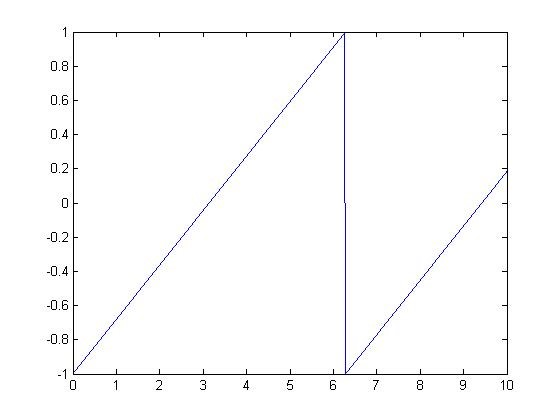
\includegraphics[height=7cm,width=8cm]{sawtooth-1.jpg}
		\caption{Sawtooth Signal}
		\label{fig:saw1}
	\end{figure}
	\par Now, you need to translate this formula to MATLAB Command : \\ $ y= sin(t) + sin(\frac{nt}{n}) $\\If we suppose that n=3,so
\begin{lstlisting}[style=Matlab-editor]
y=sin(t) + sin(3*t)/3;
plot(t,y);
\end{lstlisting}

	\begin{figure}
		\centering
		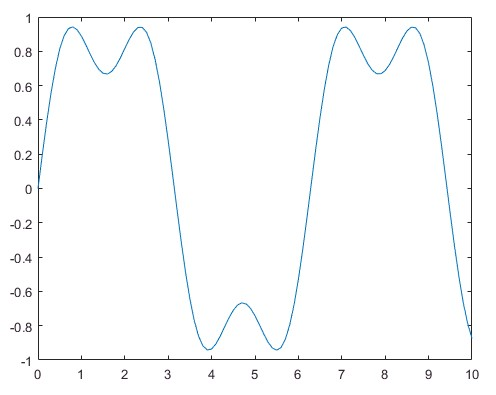
\includegraphics[width=8cm]{squarewave-2.jpg}
		\caption{Square Wave Signal 2}
		\label{fig:sw2}
	\end{figure}
	
\section{Assignment}
	\begin{enumerate}
		\item Input these n value of the Sawtooth Signal to MATLAB Command!
		\begin{itemize}
			\item n = 25
			\item n = 50 
			\item n = 75
			\item n = 100
		\end{itemize}	
	
	\item What is the output signal from Square Wave and Square Pulse below?	
	\begin{itemize}
		\item Modulate Sawtooth Signal using fm modulation. See figure \ref{lab4-code1}
		\item Modulate Sawtooth Signal using fmod and fmdemod modulation. Seefigure \ref{lab4-code2} 	
	\end{itemize}	
	
	\item Make your Conclusion about Lab Practice you did today!
	
	\clearpage
	\begin{figure}
		\centering
		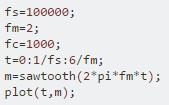
\includegraphics[width=8cm]{lab4-code1}
		\caption{Code Assignment 1}
		\label{lab4-code1}
	\end{figure}
	\begin{figure}
		\centering
		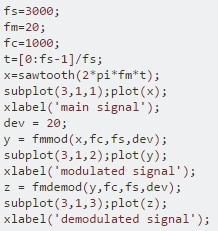
\includegraphics[width=8cm]{lab4-code2}
		\caption{Code Assignment 2}
		\label{lab4-code2}
	\end{figure}
	\clearpage
\end{enumerate}

\section{Notes}
	\par 
	Please write down your written task using Microsoft Word (format: DSP\_LAB4\_studentID.doc or docx) and the matlab code with the same name (format: DSP\_LAB4\_studentID.m ). The tasks must be finished at lab (no take home lab task), late submission of works will not be marked.

%%%%%%%%%%%%%%%%%%%%%%%%%%%%%%%%%%%%%%%%%%%%%%%%%%%%%%%%%%%%%%%%%%%%%%%%%%%%%%%%%%%%%%%%%%%%%%%%%%%%%%%%%%%%%%%%%%%%%%

\chapter{Discrete Time Signal $_{(Pt.1)}$}
\section{Objectives}
	\par 
	After a practicum assignment, it is expected that:	
	\begin{enumerate}
		\item Students can Understand the meaning of Discrete Time.
		\item Students can implement the Discrete formula into MATLAB Command.
		\item Students can Represent the output Signal of Discrete Time using MATLAB Program.
	\end{enumerate}

\section{Theory}
	\par 
	A discrete signal or discrete-time signal is a time series consisting of a sequence of quantities. In other words, it is a time series that is a function over a domain of integers.
	
	\par 
	Unlike a continuous-time signal, a discrete-time signal is not a function of a continuous argument; however, it may have been obtained by sampling from a continuous-time signal, and then arranging each value in the sequence is called a sample. When a discrete-time signal obtained by sampling a sequence corresponds to uniformly spaced times, it has an associated sampling rate; the sampling rate is not apparent in the data sequence, and so needs to be associated as a characteristic unit of the system.
	
\section{Discrete Time Signal $_{(Pt.1-Cont.)}$}
	\par To Create Signal Discrete Time by Unit Sample and Unit Step Formula
	\begin{enumerate}
	\item Unit Sample Signal
	\begin{center}
		$\delta  (n) = 
		\left \{
		\begin{tabular}{cc}
		1, & n = 0 \\
		0, & $\neq$ 0 
		\end{tabular}
		\right \} $
	\end{center}
			
	\par The command in MATLAB Program, become;
\begin{lstlisting}[style=Matlab-editor]
n = -5:5;
x = [n==0];
stem (n,x)
\end{lstlisting}
		
	\par The output signal is :
	\begin{figure}
		\centering
		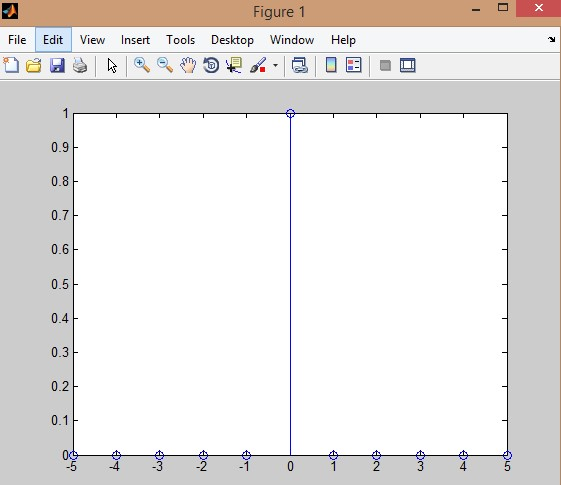
\includegraphics[width=8cm]{dt-part1.jpg}
		\caption{Discrete Time Signal 1}
		\label{fig:dt-part1}
	\end{figure}
	
	\item Unit Step Signal	
	\begin{center}
	$ \upsilon  (n) = 
	\left \{
	\begin{tabular}{cc}
	1, & n $\geq$ 0 \\
	0, & < 0 
	\end{tabular}
	\right \} $
\end{center}

	\par The command in MATLAB Program, become;
\begin{lstlisting}[style=Matlab-editor]
n = -5:5;
x = [n>0];
stem (n,x)
\end{lstlisting}

	\par The output signal is :
	\begin{figure}
		\centering
		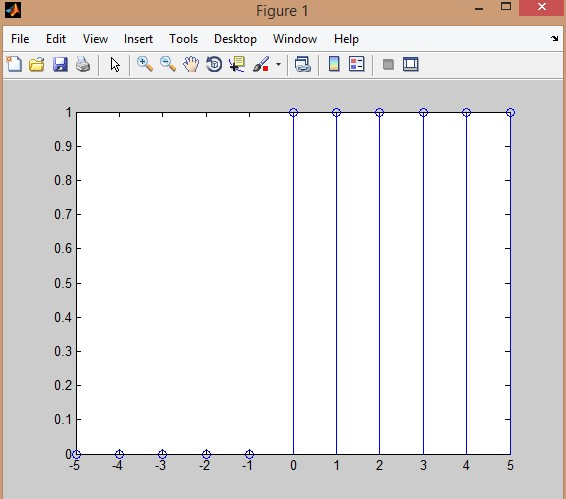
\includegraphics[width=8cm]{dt-part2.jpg}
		\caption{Discrete Time Signal 2}
		\label{fig:dt-part2}
	\end{figure}
	\end{enumerate}

\section{Assignment}
	\begin{enumerate}
		\item Change the Discreate time signal sampling and step formula below into MATLAB command!
		\begin{itemize}
			\item	
			$ \delta  (n-5) = 
			\left \{
			\begin{tabular}{cc}
			1, & n = 5 \\
			0, & n $\neq$ 5 
			\end{tabular}
			\right \} $
			
			\item 
			$ \upsilon  (n-5) = 
			\left \{
			\begin{tabular}{cc}
				1, & n $\geq$ 5 \\
				0, & n $<$ 5 
			\end{tabular}
			\right \} $
			
			\item 
			$ \upsilon_{r}  (n-1) = 
			\left \{
			\begin{tabular}{cc}
			1, & n $\geq$ 1 \\
			0, &n  $<$ 1
			\end{tabular}
			\right \} $
			
			\item 
			$ \upsilon_{r}  (n-2) = 
			\left \{
			\begin{tabular}{cc}
			n-2,& n $\geq$ 2 \\
			0,  & n $<$ 2
			\end{tabular}
			\right \} $
		\end{itemize}	
	
		\item What is the output signal from the MATLAB Command below?
		\begin{itemize}
			\item See figure \ref{lab5-code1}		
			\item See figure \ref{lab5-code2}
		\end{itemize}	
		
		\item Make your Conclusion about Lab Practice you did today!
		
		\clearpage% Flush earlier floats (otherwise order might not be correct)
		\par 
		\begin{figure}
			\centering
			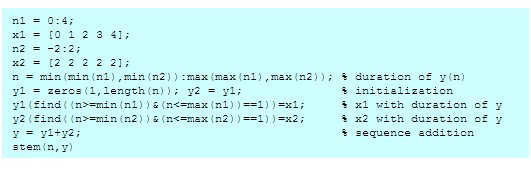
\includegraphics{lab5-code1}
			\caption{Code Assignment 1}
			\label{lab5-code1}
		\end{figure}
		\begin{figure}
			\centering
			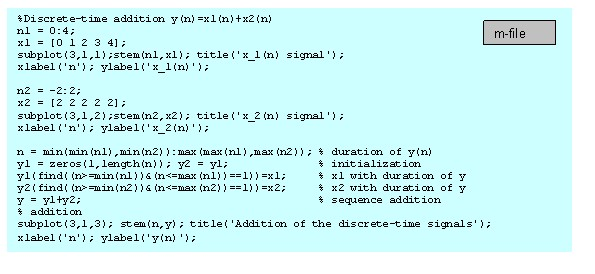
\includegraphics{lab5-code2}
			\caption{Code Assignment 2}
			\label{lab5-code2}
		\end{figure}
	 	\clearpage% Flush earlier floats (otherwise order might not be correct)
\end{enumerate}

\section{Notes}
	\par 
	Please write down your written task using Microsoft Word (format: DSP\_LAB5\_studentID.doc or docx) and the matlab code with the same name (format: DSP\_LAB5\_studentID.m ). The tasks must be finished at lab (no take home lab task), late submission of works will not be marked.

%%%%%%%%%%%%%%%%%%%%%%%%%%%%%%%%%%%%%%%%%%%%%%%%%%%%%%%%%%%%%%%%%%%%%%%%%%%%%%%%%%%%%%%%%%%%%%%%%%%%%%%%%%%%%%%%%%%%%%

\chapter{Discrete Time Signal $_{(Pt.2)}$}
\section{Objectives}
	\par 
	After a practicum assignment, it is expected that:	
	\begin{enumerate}
		\item Students can Understand the meaning of Discrete Time.
		\item Students can implement the Discrete formula into MATLAB Command.
		\item Students can Represent the output Signal of Discrete Time using MATLAB Program.
	\end{enumerate}

\section{Theory}
	\par 
	Discrete time signals are “the signals or quantities that can be defined and represented at certain time instants of the sequence.” These are finite or countable sets of number sequences. They are also called digitalized signals. A discrete signal is shown in Figure 1.
	\begin{figure}
		\centering
		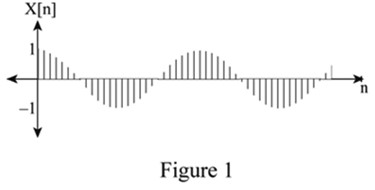
\includegraphics[width=8cm]{dt2-part1.jpg}
		\caption{Discrete Time Signal 1}
		\label{fig:dt2-part1}
	\end{figure}
	
	\par 
	One of the fundamental problems in signal processing is to obtain a permanent record of the signal itself.
	The problem with these analog recordings is that they are not abstract signals but a conversion of a physical phenomenon into another physical phenomenon: the temperature, for instance, is converted into the amount of ink on paper while the sound pressure wave is converted into the physical depth of the groove. The advent of electronics did not change the concept: an audio tape, for instance, is obtained by converting a pressure wave into an electrical current and then into a magnetic deflection. The fundamental consequence is that, for analog signals, a different signal processing system needs to be designed explicitly for each specific form of recording.
	\begin{figure}
		\centering
		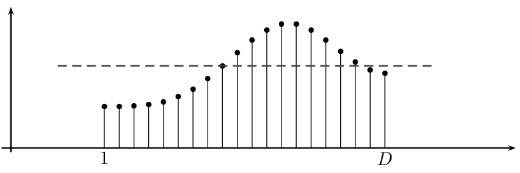
\includegraphics[width=8cm]{dt2-part2.jpg}
		\caption{Discrete Time Signal 2}
		\label{fig:dt2-part2}
	\end{figure}

\section{Discrete Time Signal $_{(Pt.2-Cont.)}$}
	\par To Create Signal Discrete Time by Unit Complex-valued and Unit Sine and Cosine Formula
	\begin{enumerate}
		\item Unit Complex-valued Exponential Signal 
		\begin{center}
			$ x(n) = e^{(\varrho + j0)n} $
		\end{center}
		
		\par The command in MATLAB Program, become;
\begin{lstlisting}[style=Matlab-editor]
n = -5:40;
x = (exp((3*4j)*n)).*[n>=0];
y = real(x);
subplot(2,1,1);
stem (n,y)
z = imag(x);
subplot(2,1,2);
stem (n,z)
\end{lstlisting}
		
		\par The output signal is :
		\begin{figure}
			\centering
			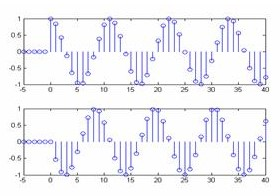
\includegraphics[width=10cm]{dt2-part3.jpg}
			\caption{Discrete Time Signal 1}
			\label{fig:dt2-part3}
		\end{figure}
			
		\begin{center}
			$ x(n) = 4 * cos (0.1\pi n + \frac{pi}{3}) $
		\end{center}
		
		\par The command in MATLAB Program, become;
\begin{lstlisting}[style=Matlab-editor]
n = -5:40;
x = 4*cos(0.1.pi*+pi/3);
stem (n,x)
\end{lstlisting}
		
		\par The output signal of the command is :
		\begin{figure}
			\centering
			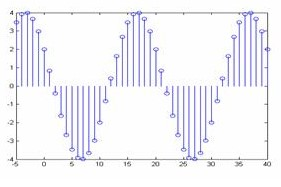
\includegraphics[width=10cm]{dt2-part4.jpg}
			\caption{Discrete Time Signal 2}
			\label{fig:dt2-part4}
		\end{figure}
	\end{enumerate}
	
\section{Assignment}
	\begin{enumerate}
		\item Change the Discreate time signal Sine and Cosine formula below into MATLAB command!
		\begin{itemize}
			\item	
			$ x(n) = 5cos(0.1\pi n + \frac{\pi}{4}) + 4sin(0.3\pi n + \frac{\pi}{4}) $
			
			\item 
			$ x(n) = 2sin(0.3\pi n + \frac{\pi}{3}) + 4sin(0.2\pi n + \frac{\pi}{4}) $
			
			\item 
			$ x(n) = 3 * cos(0.5\pi n + \frac{\pi}{3}) + 4sin(0.3\pi n + \frac{\pi}{4}) $
			
			\item 
			$ x(n) = 4 * sin(0.4\pi n + \frac{\pi}{3}) + 4sin(0.3\pi n + \frac{\pi}{4}) $
		\end{itemize}	
	
		\item What is the output signal from the MATLAB Command below?
		\begin{itemize}
			\item See figure \ref{lab6-code1}		
			\item See figure \ref{lab6-code2}
		\end{itemize}	
		
		\item Make your Conclusion about Lab Practice you did today!
	
		\clearpage% Flush earlier floats (otherwise order might not be correct)
		\par 
		\begin{figure}
			\centering
			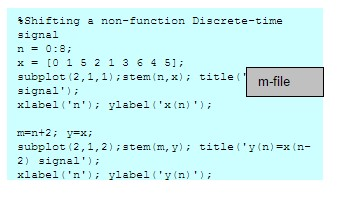
\includegraphics{lab6-code1}
			\caption{Code Assignment 1}
			\label{lab6-code1}
		\end{figure}
		\begin{figure}
			\centering
			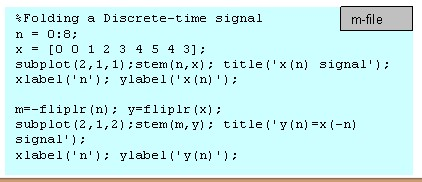
\includegraphics{lab6-code2}
			\caption{Code Assignment 2}
			\label{lab6-code2}
		\end{figure}
		\clearpage% Flush earlier floats (otherwise order might not be correct)
	\end{enumerate}

\section{Notes}
	\par 
	Please write down your written task using Microsoft Word (format: DSP\_LAB6\_studentID.doc or docx) and the matlab code with the same name (format: DSP\_LAB6\_studentID.m ). The tasks must be finished at lab (no take home lab task), late submission of works will not be marked.

\end{document}  